\documentclass[a4paper,11pt]{article}

\usepackage[english,greek]{babel}

\newcommand{\lt}{\latintext}
\newcommand{\gt}{\greektext}

\usepackage{amsmath}
\usepackage[pdftex]{graphicx}
\usepackage{verbatim}  
\usepackage[section] {placeins}
\usepackage{multirow}
\usepackage{graphicx}

\title{Προαιρετική Εργασία}
\author{Όνοματεπώνυμο: Γεώργιος Κεσογλίδης  \\  ΑΕΜ: 3911}
\date{\today}                                     

\begin{document}

\maketitle

\vspace*{1 cm}
\section{Πρώτη Άσκηση}
\vspace*{1 cm}
	\begin{center} 
		\textit{\tiny{Α}\scriptsize{Β}\footnotesize{Γ}\small{Δ}\normalsize{Ε}\large{Ζ}\Large{Η}\LARGE{Θ}\huge{I}\huge{κ}\LARGE{λ}\Large{μ}\large{ν}\normalsize{ξ}\small{ο}\footnotesize{π}\scriptsize{ρ}\tiny{σ}}
	\end{center}

\vspace*{2 cm}
\section{Δεύτερη Άσκηση}
\vspace*{1 cm}
	\begin{center} 
		\textit{ \huge{\lt Normal Italics \textbf{Bold} \\ \emph{E}mphasized \textit{\underline{Underlined}}}}
	\end{center}

\vspace*{4 cm}
\section{Τρίτη Άσκηση}
\vspace*{1 cm}
  	\begin{equation*}
		a^2+b^2=c^2
	\end{equation*}
	\begin{equation*}
		e^i\pi=-1
	\end{equation*}
	\begin{equation*}
		\pi = \frac{c}{d}
	\end{equation*}
	\begin{equation*}
		\frac{d}{dx} \int_{a}^{x} f(s) \,ds = f(x)
	\end{equation*}
	\begin{equation*}
		f(x)= \sum_{i=0}^{\infty} \frac{f^{(i)}(0)}{i!}x^i
	\end{equation*}
	\begin{equation*}
		\mathbf{Ax = b}
	\end{equation*}
	\begin{equation*}
		||x +y|| \leq ||x||+||y||
	\end{equation*}
	\vspace*{1 cm}
	\begin{equation}
		\mathbf{I} = \begin{pmatrix}
			1&0&0&0\\
			0&1&0&0\\
			0&0&1&0\\
			0&0&0&1\\
		\end{pmatrix} 
	\end{equation}
	\vspace*{1 cm}
	\begin{equation}
		\mathbf{I} = \begin{bmatrix}
			1&0&0&0\\
			0&1&0&0\\
			0&0&1&0\\
			0&0&0&1\\
		\end{bmatrix} 
	\end{equation}
	\vspace*{1 cm}
	\begin{equation}
		\mathbf{I} = \begin{Bmatrix}
			1&0&0&0\\
			0&1&0&0\\
			0&0&1&0\\
			0&0&0&1\\
		\end{Bmatrix}, \qquad \ \ 
		\mathbf{I} = \begin{vmatrix}
			1&0&0&0\\
			0&1&0&0\\
			0&0&1&0\\
			0&0&0&1\\
		\end{vmatrix}, \qquad \ \ 
		\mathbf{I} = \begin{Vmatrix}
			1&0&0&0\\
			0&1&0&0\\
			0&0&1&0\\
			0&0&0&1\\
		\end{Vmatrix}  
	\end{equation}

\section{Τέταρτη Άσκηση}
\vspace*{1 cm}
  \begin{center}
	\it {
	\begin{tabular}{ l c r }
  		Τέφας & 2 & 3 \\
  		Πήτας & 5 & 6 \\
  		Λάσκαρης & 8 & 9 \\
	\end{tabular}
\vspace*{1 cm}\\
	\begin{tabular}{| l | c | r |}
  		Κοτρόπουλος & 6 & 3 \\
  		Πήτας & 5 & 6 \\
  		Νικολαίδης & 8 & 9 \\
	\end{tabular}
\vspace*{1 cm}\\
	\begin{tabular}{ | l | c | r |}
    	\hline
    	1 & 2 & 3 \\ \hline
    	4 & 5 & 6 \\ \hline
    	7 & 8 & 9 \\ 
    	\hline
  	\end{tabular}
\vspace*{1 cm}\\
  	\begin{tabular}{ | l | c | r |}
    	\hline
    	1 & 2 & 3 \\ \hline
    	4 & 5 & 6 \\ \hline
    	7 & 8 & 9 \\ 
    	\hline
  	\end{tabular}
\vspace*{1 cm}\\
  	\begin{tabular}{| l | l |  l |}
  		\hline
  		\multicolumn{3}{|c|}{Μέλη ΔΕΠ Πληροφορικής} \\
  		\hline
 		Λέκτορες & \lt VD & Δραζιώτης Κωνσταντίνος \\
 		\hline
 		\multirow{2}{*}{Επίκουροι} & \lt LN & Λάσκαρης Νικόλαος \\ 
 		& \lt TG & Τσουμάκας Γρηγόριος \\ 
 		\hline
 		\multirow{3}{*}{Αναπληρωτές} & \lt TA & Τέφας Αναστάσιος \\ 
 		& \lt PN & Πλέρος Νίκος \\ 
 		& \lt PA & Παπαδόπουλος Απόστολος \\ 
 		\hline
 		\multirow{3}{*}{Καθηγητές} & \lt KC & Κοτρόπουλος Κωνσταντίνος \\ 
 		& \lt PI & Πήτας Ιωάννης \\ 
 		& \lt VI & Βλαχάβας Ιωάννης \\ 
 		\hline

	\end{tabular}}
  \end{center}   

\vspace*{2 cm}

\section{Πέμπτη Άσκηση}
	\vspace*{1 cm}
\it{
\begin{itemize}
   \item Τέφας
   \item Μπουζάς
   \item Μπρούζα
   \item Λάσκαρης
   \item Κοτρόπουλος
   \item Πήτας
   \item Νικολαΐδης
\end{itemize}
\begin{enumerate}
   \item Τέφας
   \item Μπουζάς
   \item Μπρούζα
   \item Λάσκαρης
   \item Κοτρόπουλος
   \item Πήτας
   \item Νικολαΐδης
\end{enumerate}
\begin{description}
   \item[\bf{(α)}] Τέφας
   \item[\bf{(β)}] Μπουζάς
   \item[\bf{(γ)}] Μπρούζα
   \item[\bf{(δ)}] Λάσκαρης
   \item[\bf{(ε)}] Κοτρόπουλος
   \item[\bf{(ζ)}] Πήτας
   \item[\bf{(η)}] Νικολαΐδης
\end{description}
}

\section{Έκτη Άσκηση}

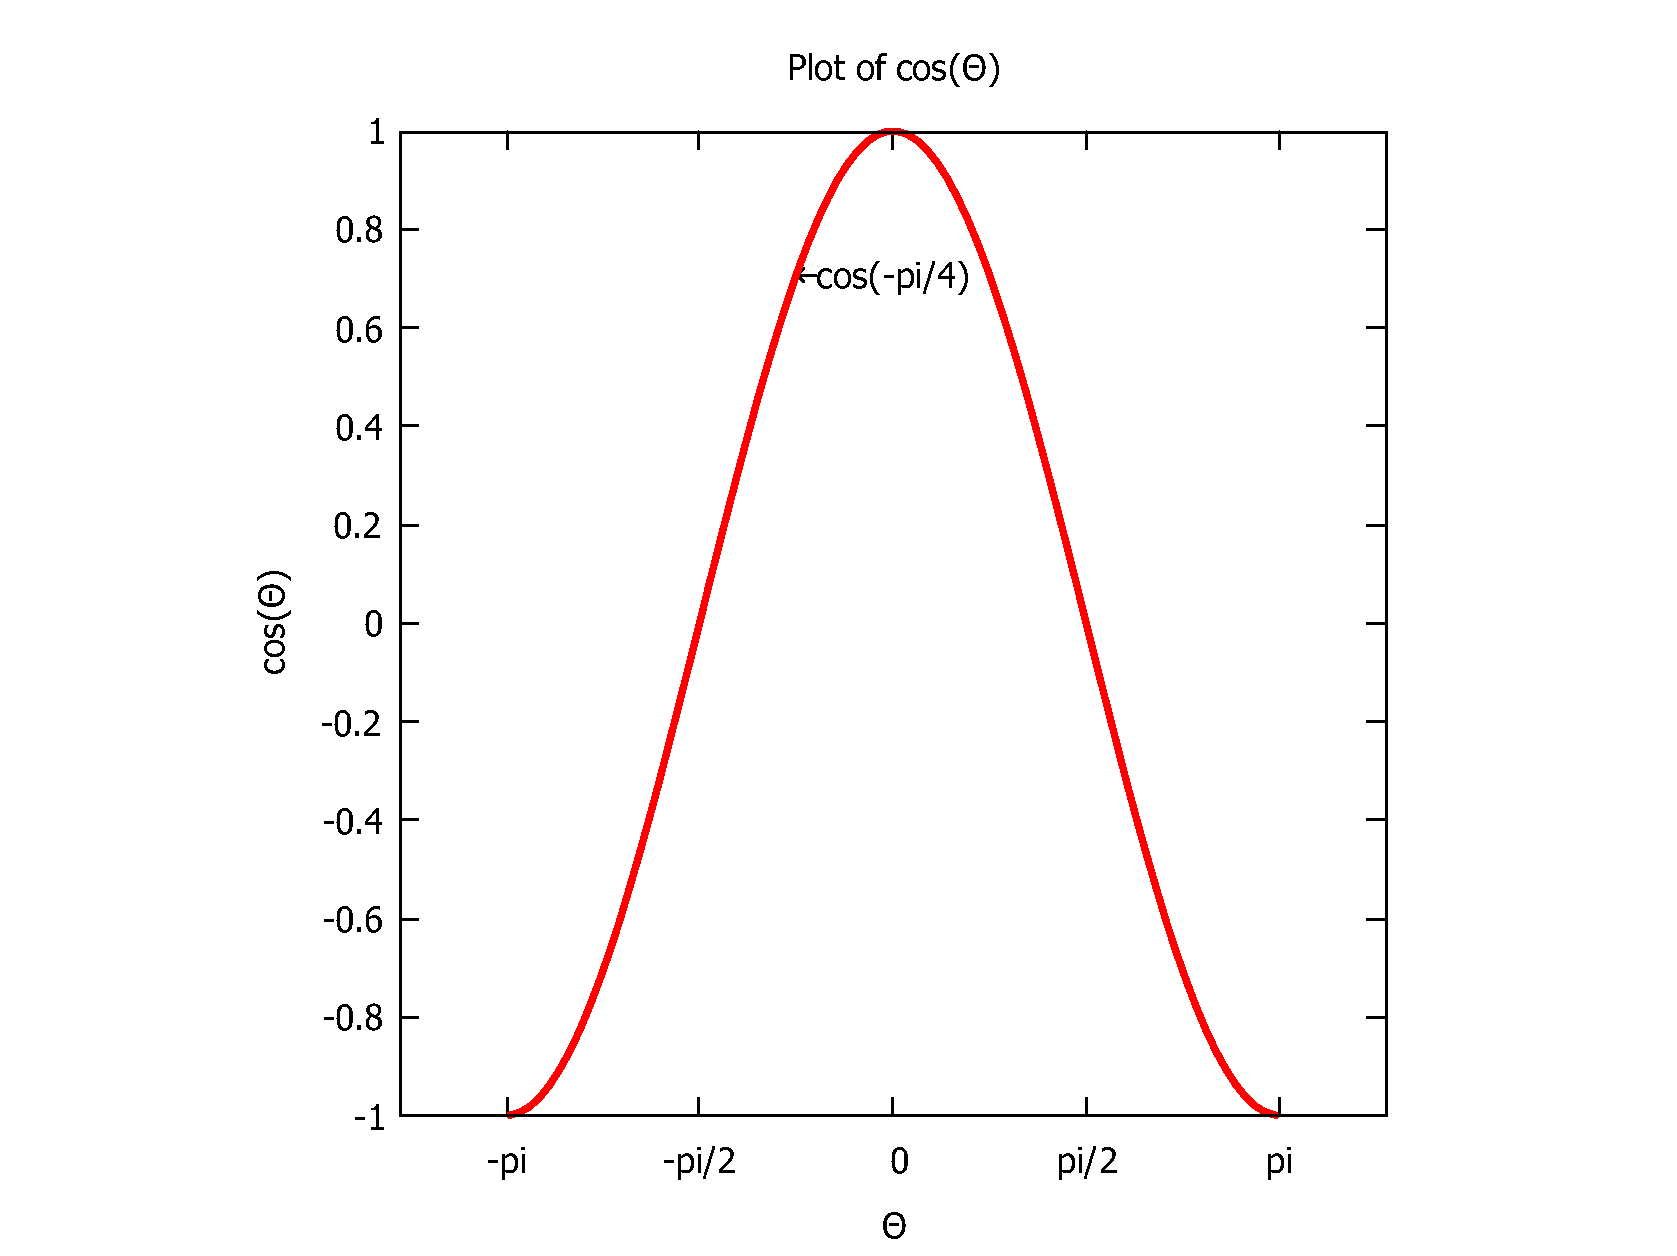
\includegraphics[height=9cm, width=12cm]{cos(th).pdf}

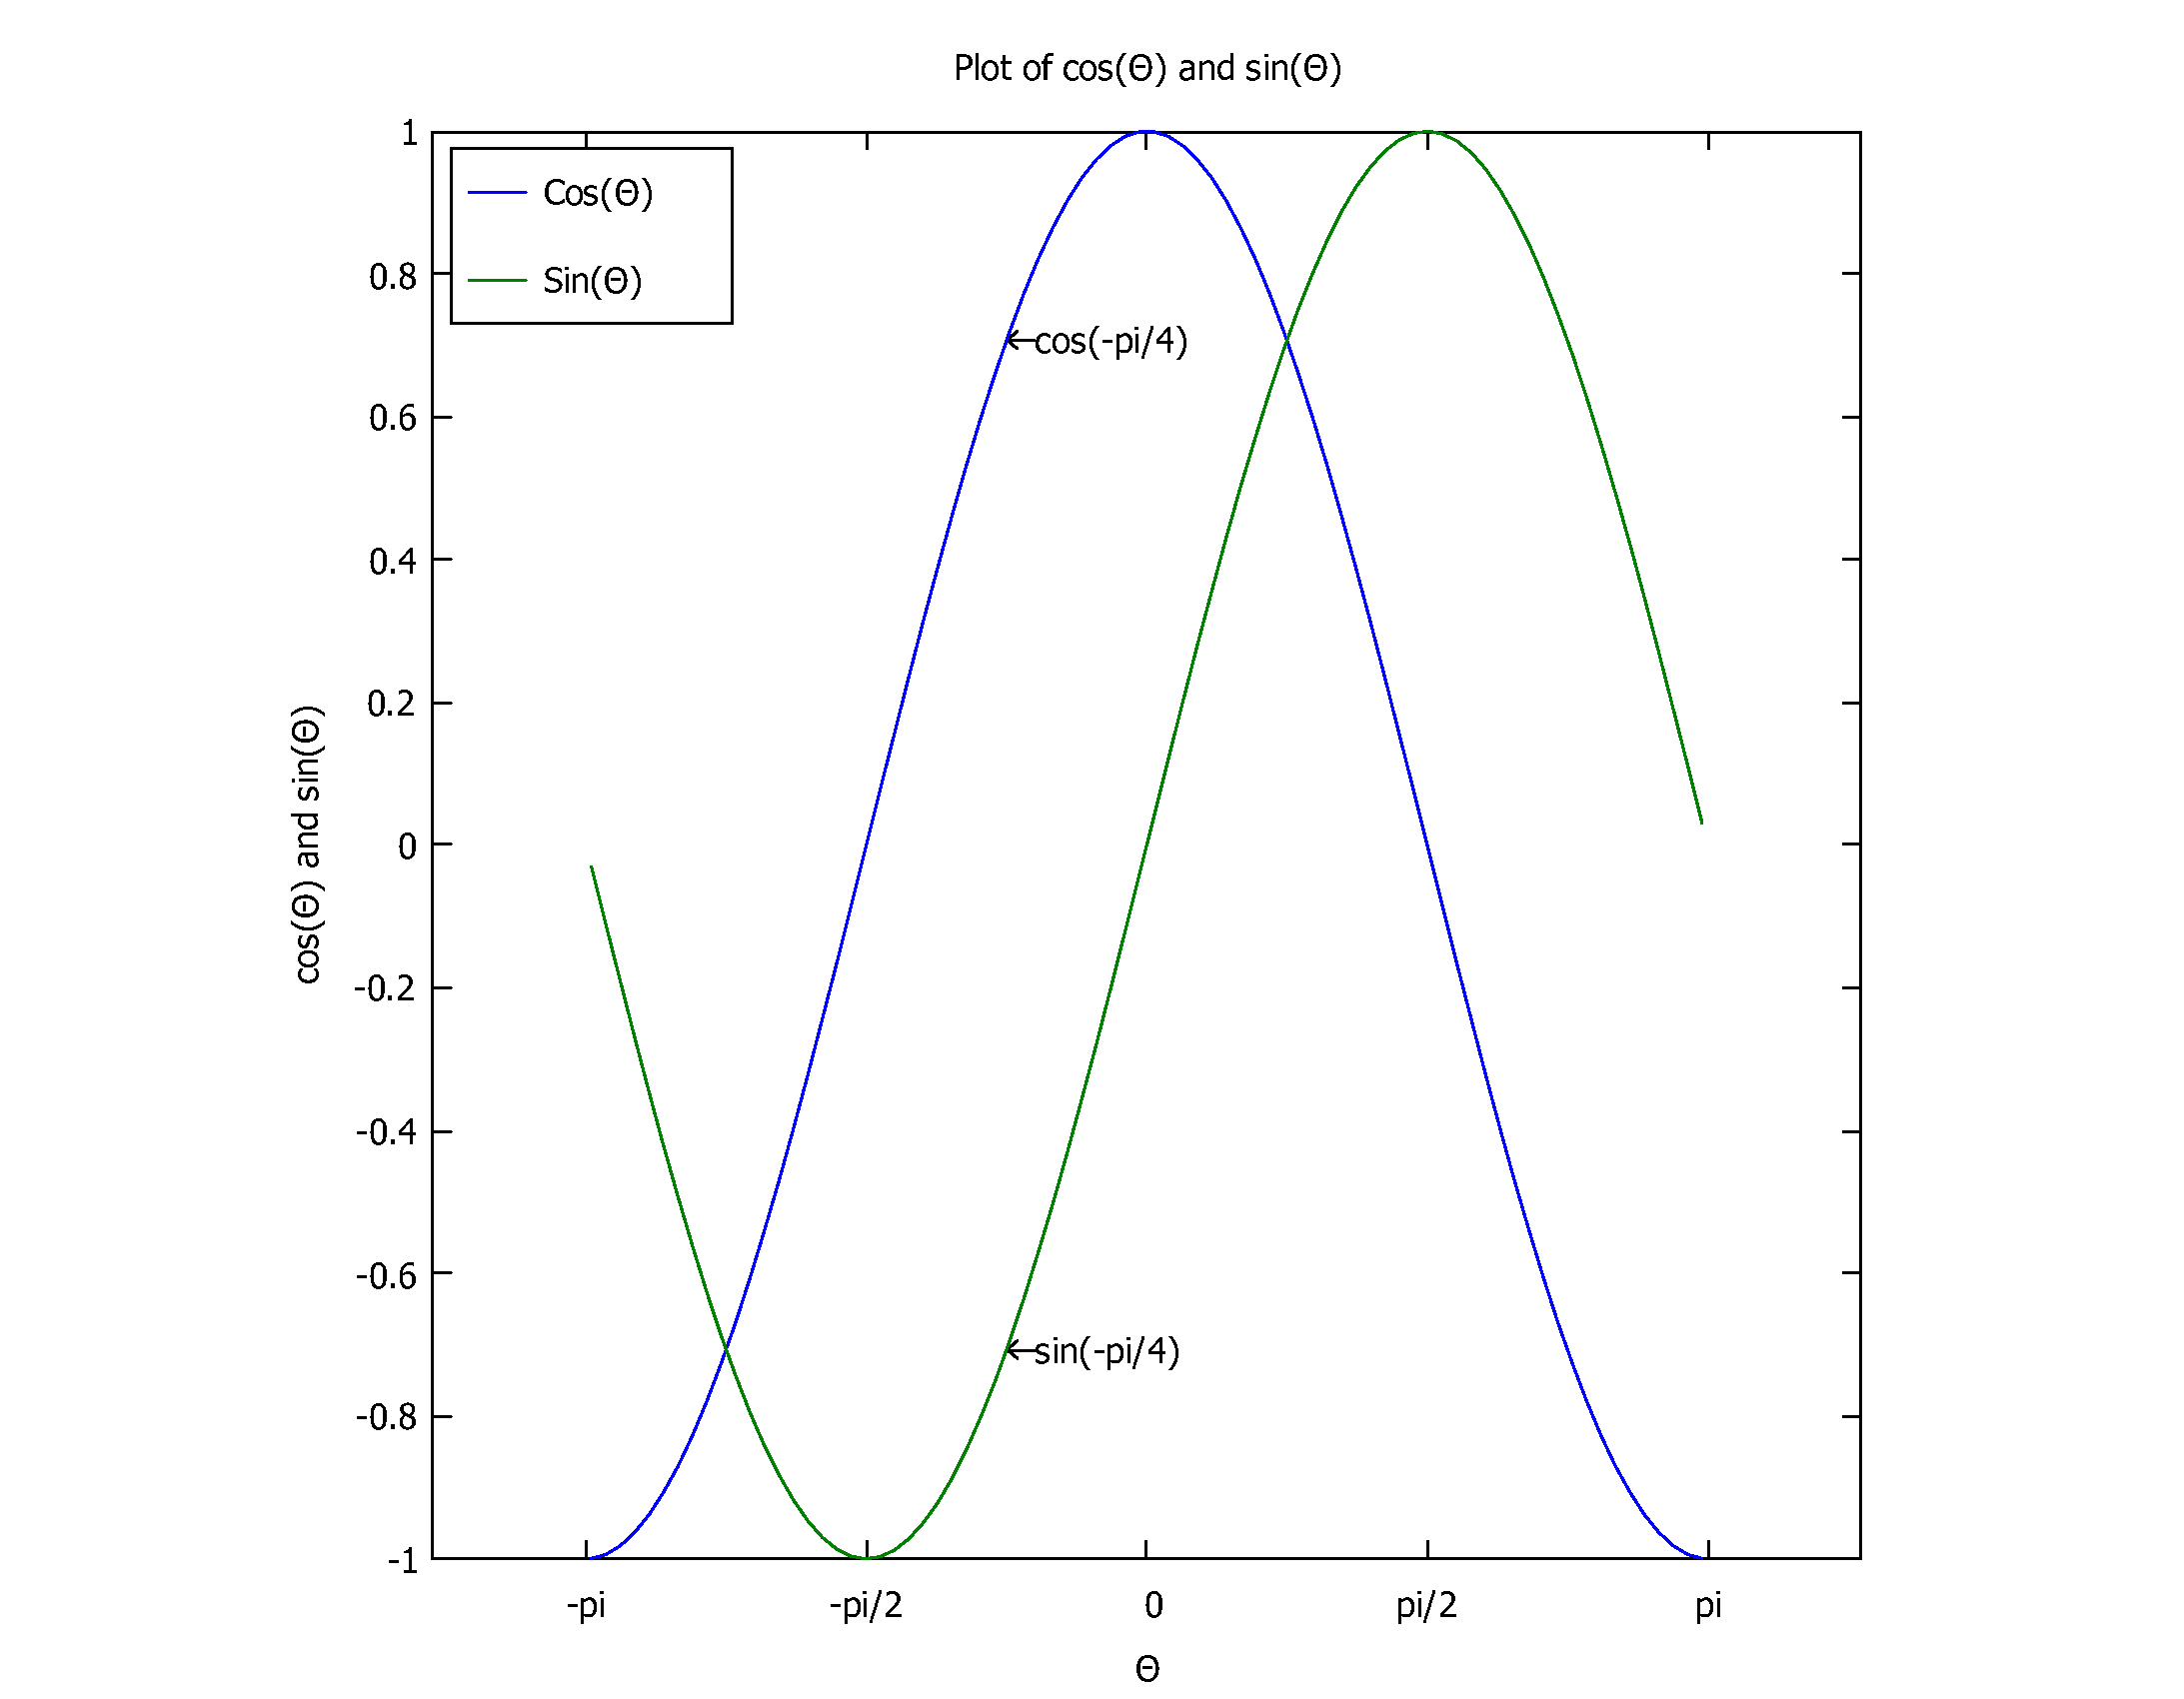
\includegraphics[height=9cm, width=11cm]{sin(th).pdf}

\end{document}
